\chapter{Design}\label{chapter:design}

This chapter explains how we designed the monitoring infrastructure. The
design starts from the feature model that we developed to answer RQ2. We used
the model as a map of the design space rather than as an implementation
checklist: it made clear which parts of ROS~2 monitoring could reasonably fit
into one thesis prototype and which parts should remain outside the scope.

\section{Feature Model as Design Input}

Figure~\ref{fig:feature-model} shows the feature model. It
organizes ROS~2 monitoring along several dimensions: observable elements,
monitoring architecture, monitoring mode, system configuration, and
implementation paradigm. When we built this model, the main lesson was that
``monitoring ROS~2'' is too broad to be treated as one feature. A monitor may
observe topics, services, actions, parameters, node states, or middleware
events. It may run centrally or in several places. It may be passive or active.
It may be implemented as a normal ROS~2 monitor node, as an inserted decorator,
as a network tap, or through lower-level middleware and tracing tools.

\begin{figure}[htbp]
    \centering
    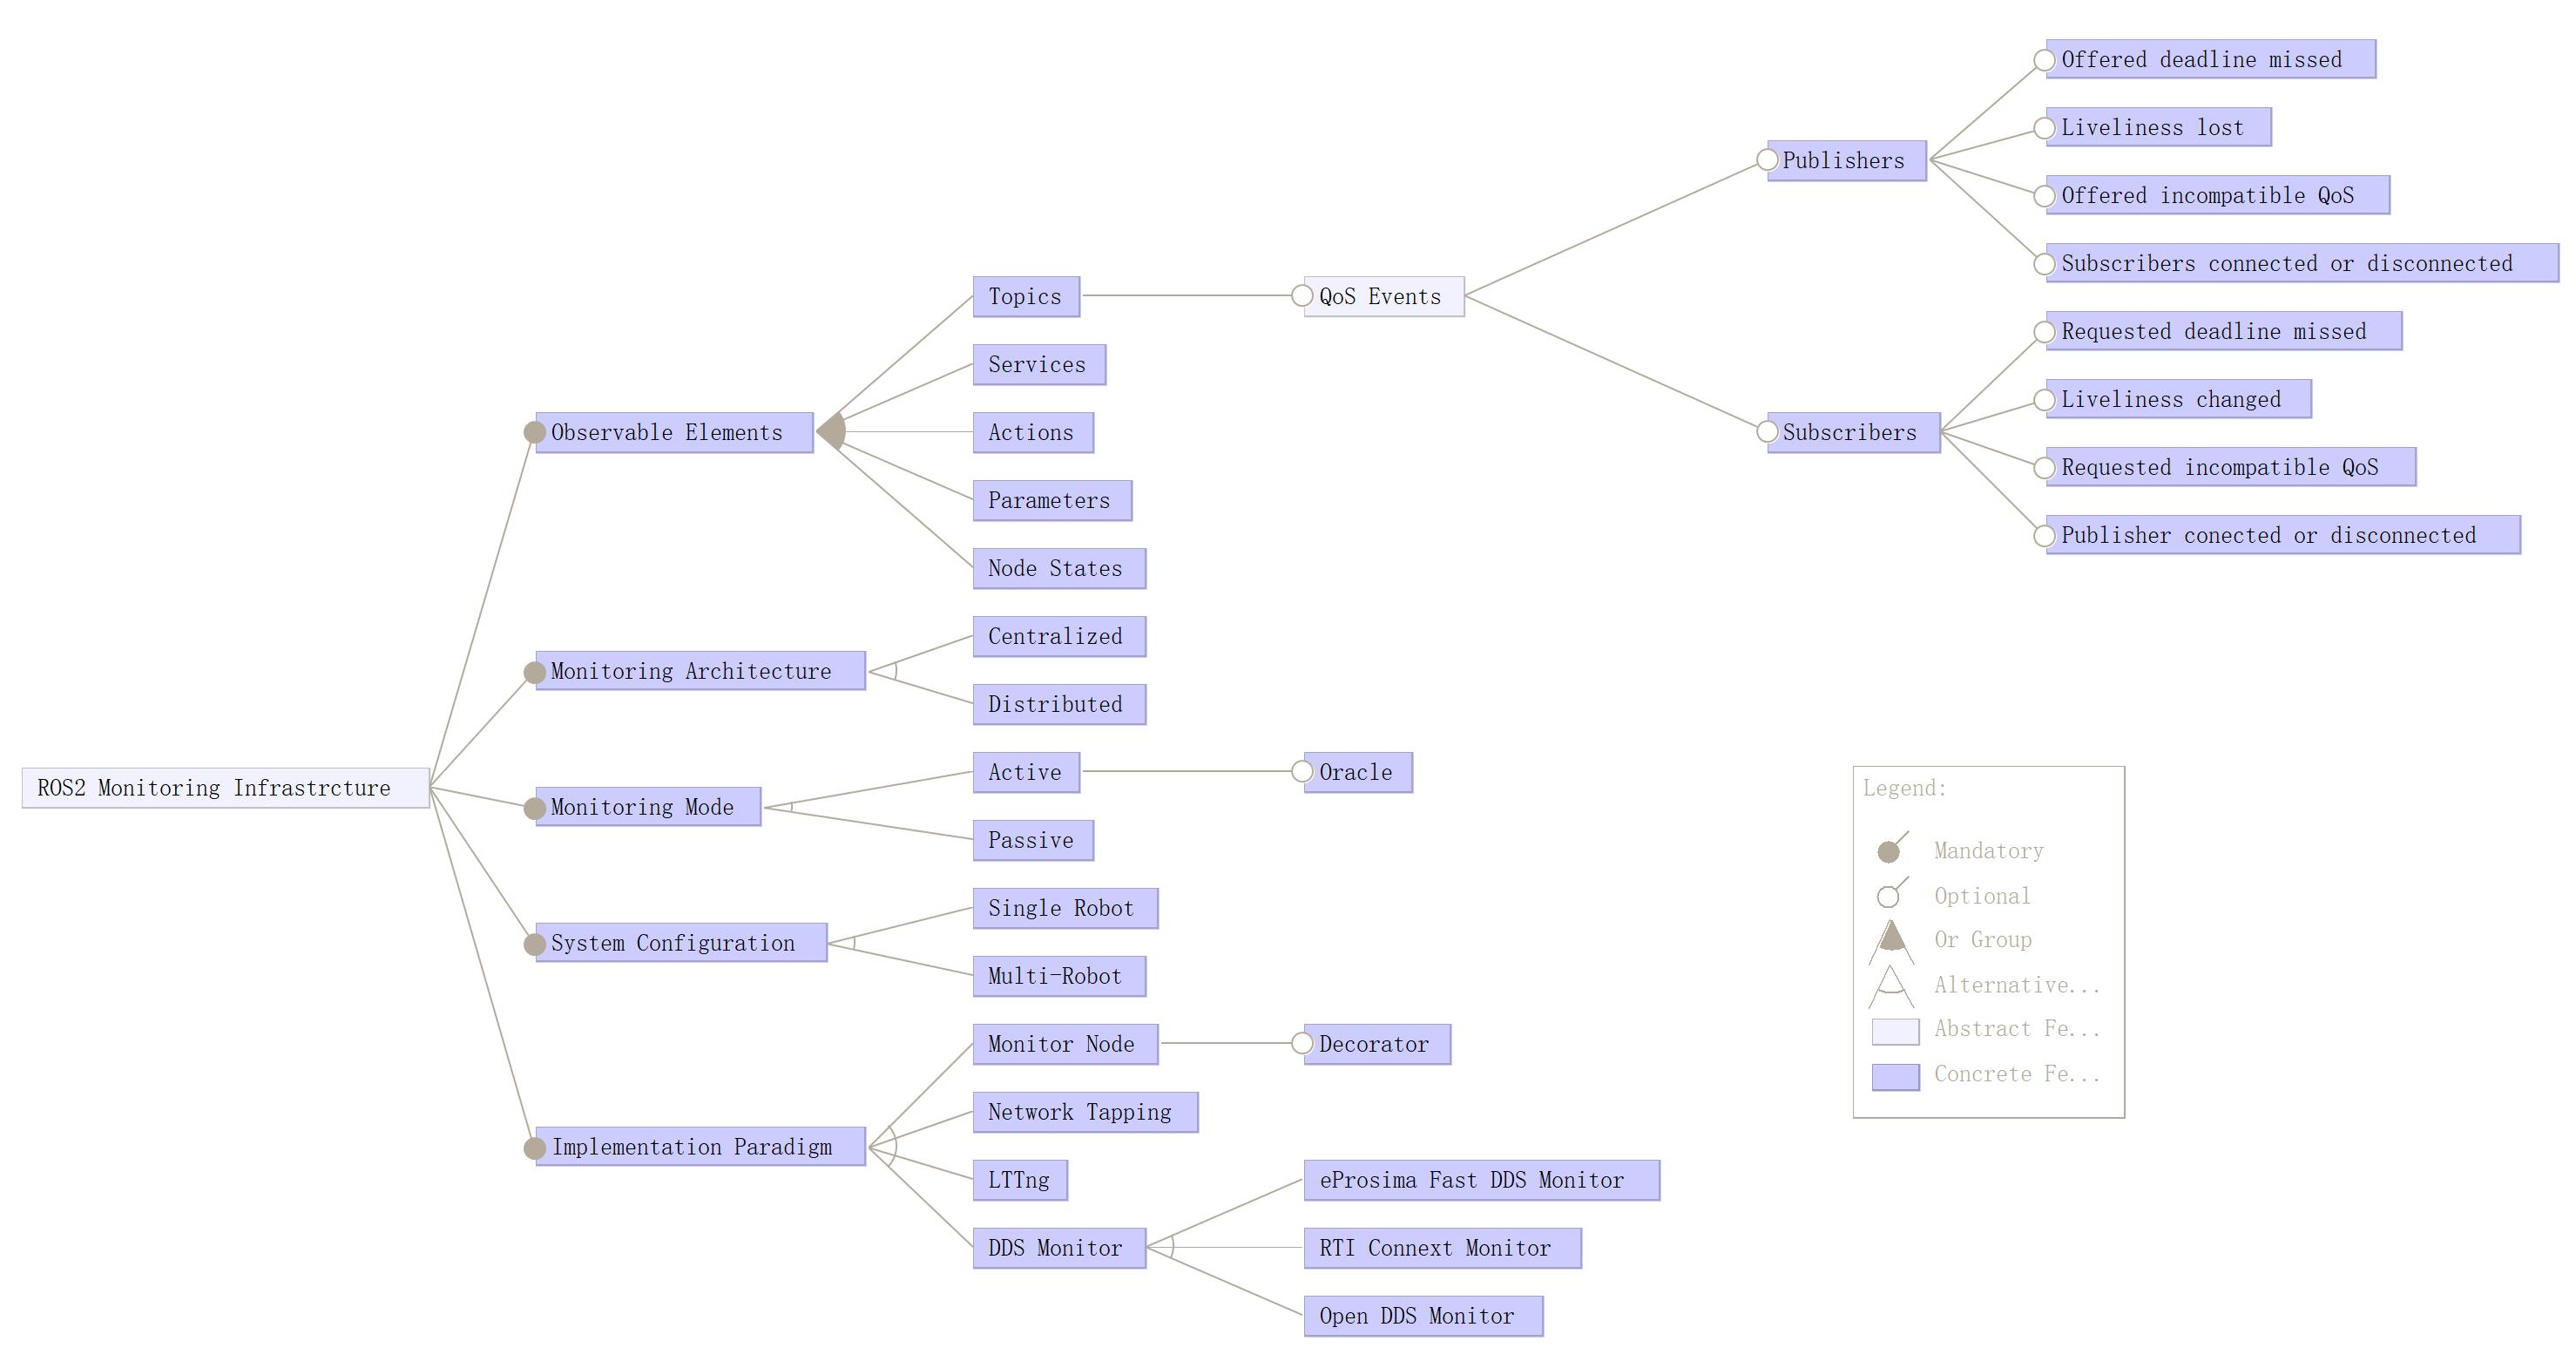
\includegraphics[width=\textwidth]{diagrams/FeatureModel.jpg}
    \caption{Feature model of the ROS~2 monitoring infrastructure domain,
    using the notation introduced in Section~\ref{sec:feature-models}.}
    \label{fig:feature-model}
\end{figure}

The concrete prototype implements one path through this map: application-level
data that can be collected passively, represented in a common format, and
configured without rewriting the monitoring core.

\section{Selected Feature Coverage}

Table~\ref{tab:selected-feature-coverage} summarizes how the implemented
prototype relates to the feature model. The table distinguishes between
features that are implemented directly, features that are represented by the
demonstration scenarios, and features that remain outside the current design.

\begin{table}[htbp]
\centering
\begin{tabular}{
    >{\raggedright\arraybackslash}p{0.24\textwidth}
    >{\raggedright\arraybackslash}p{0.34\textwidth}
    >{\raggedright\arraybackslash}p{0.32\textwidth}
}
\toprule
\textbf{Feature dimension} &
\textbf{Selected coverage} &
\textbf{Not covered in the prototype} \\
\midrule
Observable elements &
Topics, service request and response events, and action feedback and status are
collected as typed ROS~2 observations. &
Parameters, node lifecycle states, DDS-level QoS events, network packets, and a
complete action trace with goal, cancellation, and result events. \\
\midrule
Monitoring architecture &
The infrastructure supports an integrated setup and a split robot/verifier
setup. Demo scenarios also exercise hybrid, multi-robot, global, choreographed,
and offline replay organizations. &
Automatic monitor placement, fault-tolerant distributed verification, global
message ordering, and clock synchronization guarantees. \\
\midrule
Monitoring mode &
Monitoring is passive: the prototype observes data and produces records and
verdicts. &
Active intervention, automatic recovery, message blocking, or changes to robot
behaviour. \\
\midrule
System configuration &
Single-robot and multi-robot configurations can be expressed with the same YAML
configuration concepts and record format. &
Automatic generation of the full monitoring configuration from a system model
or graphical tool. \\
\midrule
Implementation paradigm &
The prototype is implemented as ROS~2-facing monitor nodes plus optional
verifier-side processes. &
Decorator-based interception, network tapping, LTTng tracing, and DDS-specific
monitor implementations. \\
\bottomrule
\end{tabular}
\caption{Selected prototype coverage with respect to the feature model.}
\label{tab:selected-feature-coverage}
\end{table}

This coverage is intentionally narrower than the full feature model. The goal
is not to cover every possible monitoring technique. The goal is to build and
validate a reusable path from ROS~2 application observations to checking
components, while keeping the parts that usually change between applications
configurable.

\section{Design Requirements}

The selected feature coverage led to a few design requirements that shaped the
prototype. The most important one is the common record format. Topics, service
events, and action feedback/status should not force later components to deal
with three unrelated data shapes. The record therefore has to carry not only
the payload, but also the source, timestamp, session, and identity information
needed to connect observations with later verdicts.

We also wanted processing to happen early in the pipeline. Raw ROS~2 messages
can be large or frequent, and in many cases the checker only needs a few fields
or only needs records when values change. This pushed field extraction,
throttling, and filtering into the infrastructure before storage or transport.

The remaining requirements are about keeping changeable parts apart. Collection
needs ROS~2 type and communication knowledge without being tied to one checking
language. A converter may adapt records for a checker, while a verdict service
contains the property-specific logic. YAML configuration covers common choices,
and plugins cover project-specific conversion, checking, input, and output
behaviour. The same chain should then be usable both when everything runs in
one ROS~2-facing process and when records cross a transport boundary to a
separate verifier.

\section{Infrastructure Overview}

The infrastructure is organized as a dataflow pipeline. A collector observes
one ROS~2 source and creates a common data record. A transformer pipeline can
reduce or modify the record, for example by selecting fields, limiting the
rate, or emitting only changed values. Dispatchers then route the record to data
exporters and to optional checking chains.

Checking is deliberately separated into two steps. A converter prepares a data
record for one property-specific checker. A verdict service evaluates the
prepared data and returns a structured verdict. Verdict exporters then deliver
the result to standard output, a file, MQTT, or another configured destination.
This separation keeps the ROS~2 collection layer independent from a particular
verification language or checking algorithm.

Figure~\ref{fig:pipeline-components} shows the main pipeline stages. The same
chain is used for topic messages, service events, and action feedback or status
records, so a new source type does not require a new checking architecture.

\begin{figure}[htbp]
    \centering
    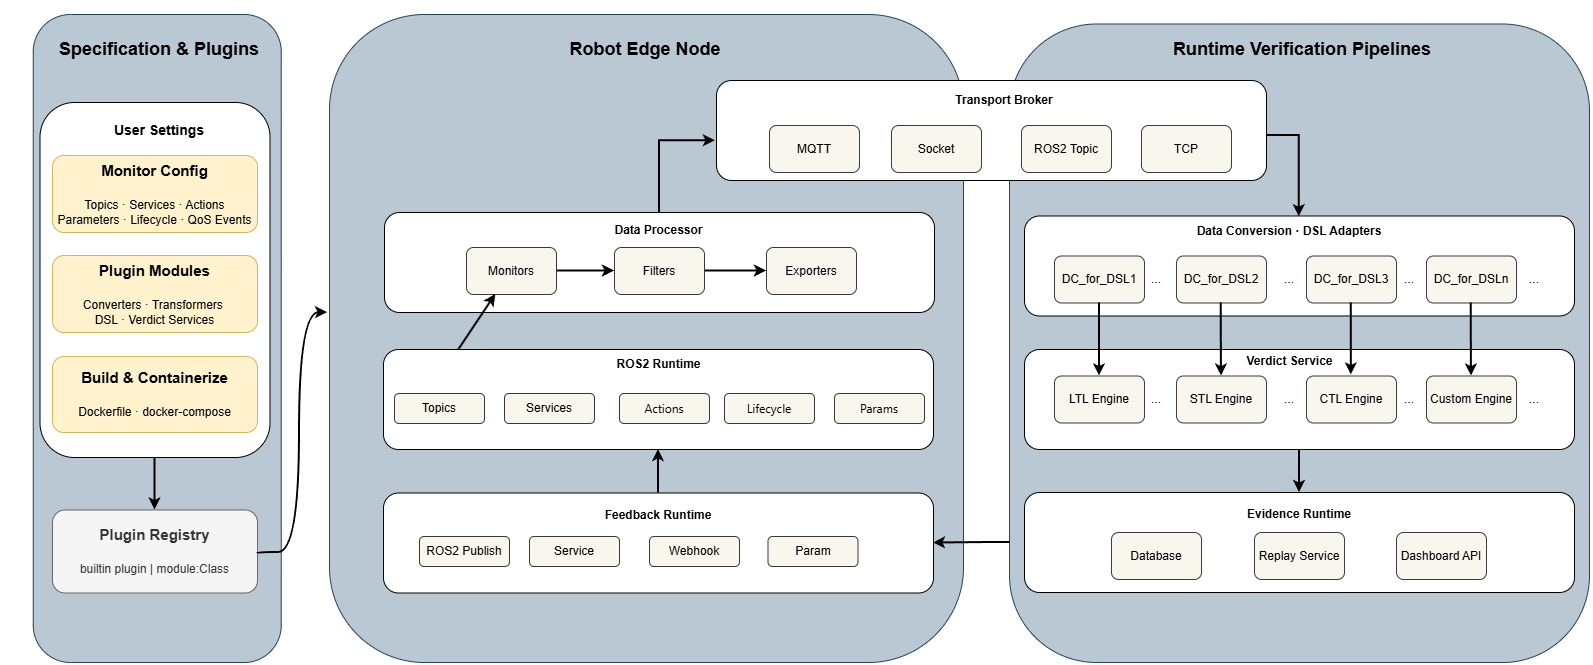
\includegraphics[width=\textwidth]{diagrams/Components.png}
    \caption{Main stages of the monitoring pipeline. Collectors create common
    data records, transformers process them, dispatchers route them, converters
    adapt them for checkers, and verdict exporters publish the checking
    results.}
    \label{fig:pipeline-components}
\end{figure}

\section{Pipeline Roles}

The implementation chapter uses several role names repeatedly. They have the
following meanings in the design:

\begin{description}
    \item[Collector] A ROS~2-facing component that subscribes to one configured
    topic, service event stream, or action feedback/status stream and turns
    each observation into a data record.

    \item[Transformer pipeline] An ordered set of processing steps that can
    remove fields, throttle records, or suppress unchanged values before data is
    stored, transported, or checked.

    \item[Dispatcher] A routing component that fans a record out to one or more
    downstream exporters or checking chains.

    \item[Data exporter] A sink for data records, such as a JSONL file, standard
    output, or MQTT topic.

    \item[Source] A verifier-side input adapter that reads data records from a
    transport or replay file and injects them into the same checking chain.

    \item[Converter] A property-specific adapter that projects a data record
    into the input shape expected by a checker.

    \item[Verdict service] A checker that evaluates converted data and returns
    a structured verdict when a property state is observed.

    \item[Verdict exporter] A sink for verdicts, such as standard output, a
    JSONL file, or an MQTT verdict topic.
\end{description}

This naming keeps the infrastructure precise: collectors and sources introduce
records, transformers change records, dispatchers route records, converters
adapt records for property logic, and verdict services perform the actual
checking.

\section{Common Data Record}

The common data record is the central abstraction of the infrastructure. Every
captured topic message, service event, and action observation is converted into
this format before it reaches processing, transport, or checking. Records are
serialized as JSONL, with one JSON object per line. Empty optional fields are
omitted from the serialized output to keep files and MQTT payloads compact.

Table~\ref{tab:data-record-schema} summarizes the fields used by the record.
The field names follow the implementation and the detailed record
specification in \texttt{docs/datarecord\_spec.md}.

\begin{table}[htbp]
\centering
\begin{tabular}{
    >{\raggedright\arraybackslash}p{0.22\textwidth}
    >{\raggedright\arraybackslash}p{0.20\textwidth}
    >{\raggedright\arraybackslash}p{0.48\textwidth}
}
\toprule
\textbf{Field} & \textbf{Presence} & \textbf{Purpose} \\
\midrule
\texttt{\_type} & All records &
Identifies the record kind: session start, data, session end, or error. \\
\midrule
\texttt{session\_id} & All records &
Groups all records produced during one monitoring run. \\
\midrule
\texttt{record\_id} & Data records &
Gives one captured observation a stable identity for correlation with later
verdicts. \\
\midrule
\texttt{source\_type} & Data records &
States whether the observation came from a topic, service, or action. \\
\midrule
\texttt{source\_name} & Data records &
Stores the logical ROS~2 name, such as \texttt{/cmd\_vel},
\texttt{/set\_bool}, or \texttt{/navigate\_to\_pose}. \\
\midrule
\texttt{source\_node} & When known &
Records the publisher or server node name found during collection. \\
\midrule
\texttt{msg\_type} & Data records &
Preserves the ROS~2 type identifier needed by downstream converters. \\
\midrule
\texttt{phase} & Services/actions &
Distinguishes request, response, feedback, status, goal, or result phases. \\
\midrule
\texttt{timestamp} & All records &
Stores the monitor-side wall-clock time when the record was created. \\
\midrule
\texttt{ros\_timestamp} & When available &
Preserves the timestamp carried by the original ROS~2 message or event. \\
\midrule
\texttt{data} & All records &
Contains the monitoring configuration, captured payload, session statistics,
or error details, depending on \texttt{\_type}. \\
\midrule
\texttt{metadata} & Data records &
Stores infrastructure context such as sequence number, QoS profile, applied
transformers, service event type, client identifier, and service sequence
number. \\
\bottomrule
\end{tabular}
\caption{Schema of the common data record used throughout the infrastructure.}
\label{tab:data-record-schema}
\end{table}

The record format is deliberately uniform across ROS~2 communication methods.
Topics have no phase because each message is a complete unit. Service events
are unwrapped into request and response records, with the service event metadata
kept for correlation. Actions use feedback and status records directly, while
goal and result phases can be represented when service introspection for those
action services is available. The same \texttt{session\_id},
\texttt{record\_id}, \texttt{source\_type}, and \texttt{source\_name} fields
therefore identify observations regardless of whether they originated from a
topic, service, or action.

\section{Deployment Topologies}

The same pipeline can run in two main deployment forms. In the integrated
deployment, collection, processing, checking, and output run in one
ROS~2-facing process. This form is useful for local development and for
properties that can be checked close to the observed application.

\begin{figure}[htbp]
    \centering
    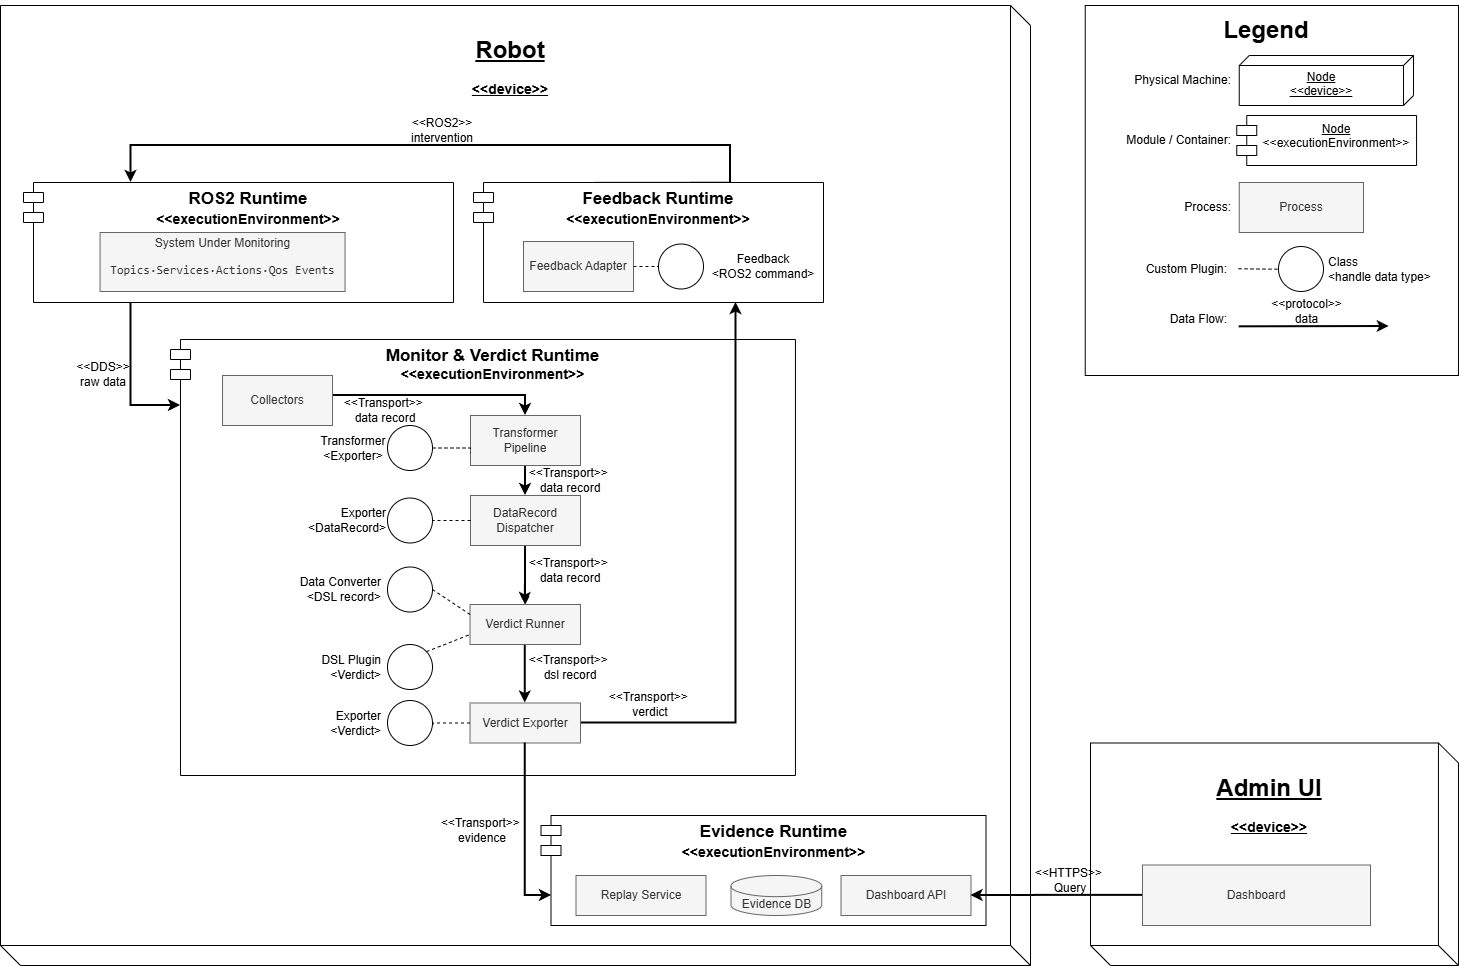
\includegraphics[width=0.72\textwidth]{diagrams/UML deployment integrated.png}
    \caption{Integrated deployment topology. Collection, processing, checking,
    and verdict export are placed in the same ROS~2-facing monitor runtime.}
    \label{fig:deployment-integrated}
\end{figure}

In the split deployment, a robot-side monitor collects and processes
observations and sends data records to a verifier-side process. The verifier
uses a source adapter to read those records and then executes the same
converter, verdict service, and verdict exporter chain that is used in the
integrated deployment. The prototype implements file replay and MQTT for these
flows, but transport remains an exporter/source choice rather than part of the
checking logic.

\begin{figure}[htbp]
    \centering
    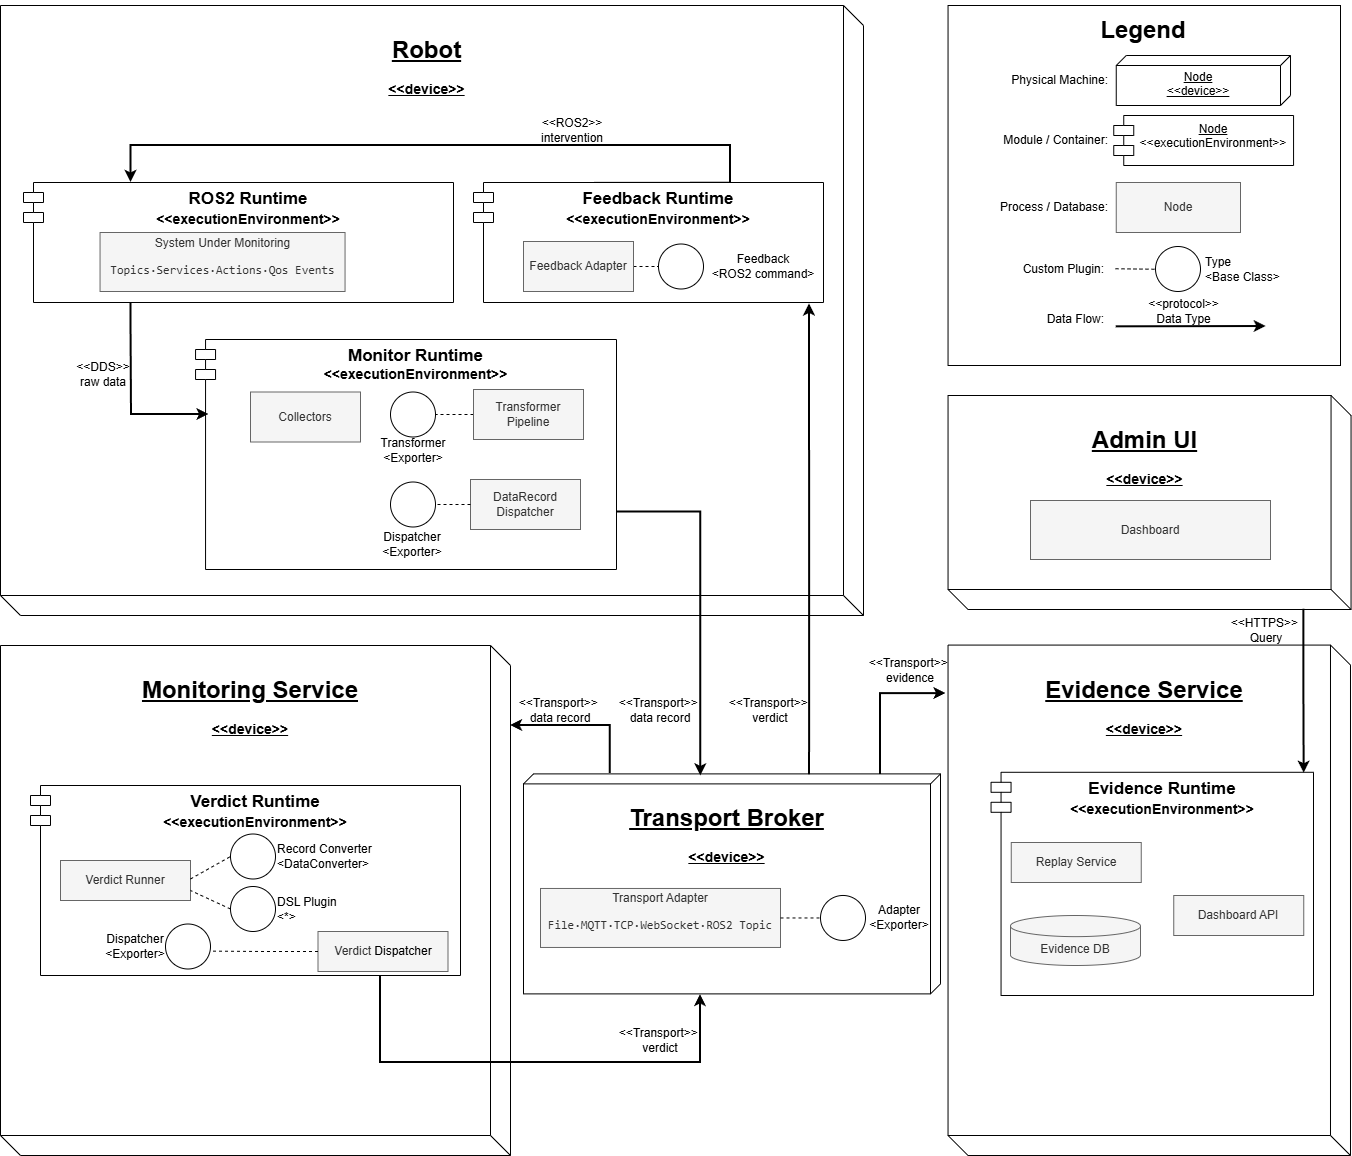
\includegraphics[width=0.72\textwidth]{diagrams/UML deployment separated.png}
    \caption{Split deployment topology. The robot-side monitor publishes data
    records through a transport boundary, while a verifier-side process runs
    the checking chain and exports verdicts.}
    \label{fig:deployment-split}
\end{figure}

Figure~\ref{fig:pipeline-sequence} shows the runtime order of the main
pipeline interactions. The sequence is the same in both deployment forms until
a data exporter or source crosses the transport boundary.

\begin{figure}[htbp]
    \centering
    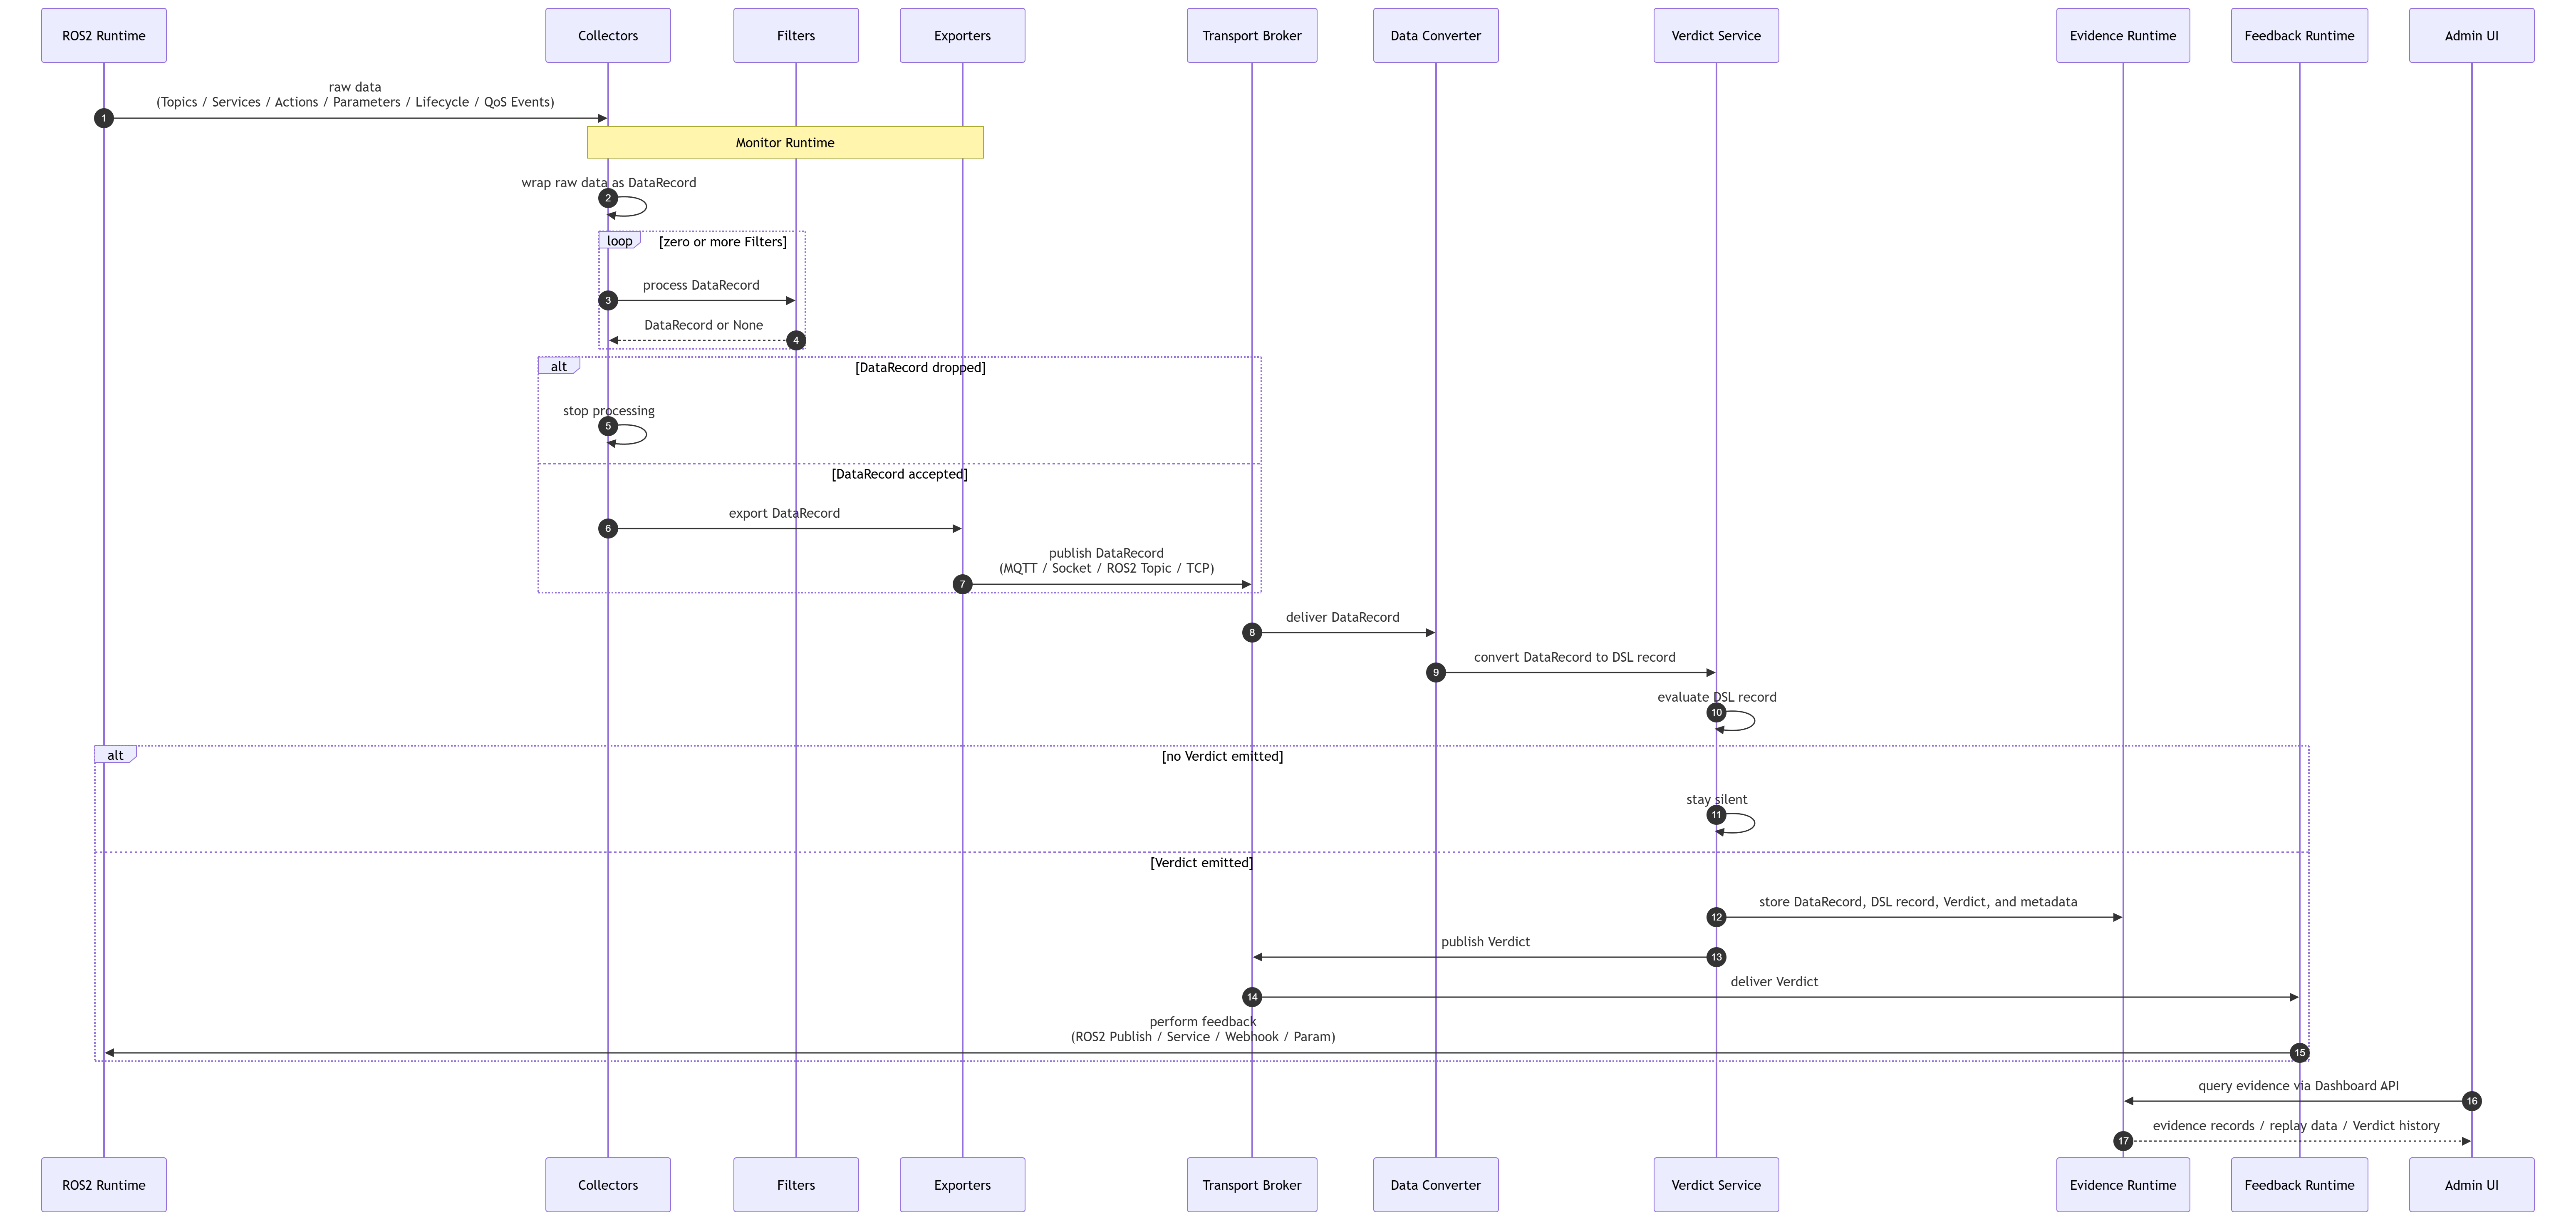
\includegraphics[width=\textwidth]{diagrams/SequenceDiagram.png}
    \caption{Runtime sequence from collection to verdict export.}
    \label{fig:pipeline-sequence}
\end{figure}
